\chapter{Em busca da Arborescência Perdida}


Vamos usar esse capítulo para situar a evolução do problema: começamos revisitando como se encontra conectividade de menor custo em grafos não dirigidos por meio de \emph{árvores geradoras mínimas} (MST), onde estratégias gulosas são corretas graças aos princípios de \emph{corte} e de \emph{ciclo}. Em seguida veremos por que, ao passar para \emph{digrafos} e buscar uma \textbf{r-arborescência de custo mínimo}, essas mesmas receitas não se aplicam literalmente: surgem ciclos dirigidos e falta um “corte seguro” direto. Essa transição motiva as ferramentas certas — \emph{custos reduzidos} e \emph{contração de ciclos} — que aparecem no algoritmo de \textbf{Chu–Liu/Edmonds} e, adiante, no procedimento em duas fases de \textbf{Frank}.

\section{Contexto Histórico}
O problema de encontrar uma r-arborescência de custo mínimo em um digrafo ponderado é de certa forma uma evolução do problema de conectividade de menor custo em grafos não dirigidos, mas traz desafios adicionais que exigem novas ferramentas e estratégias.

\subsection{A busca em grafos}


Antes de tratarmos do caso \emph{dirigido}, vamos falar sobre a intuição dominante de \emph{como construir estruturas de conectividade de menor custo} vinha do caso de \emph{grafos não dirigidos}: as \textbf{árvores geradoras mínimas}\footnote{Definição. Em um grafo não dirigido, conexo e ponderado \(G=(V,E)\) com pesos \(w:E\to\mathbb{R}\), uma árvore geradora mínima é um subconjunto de arestas \(T\subseteq E\) que forma uma árvore (conecta todos os vértices, é acíclica e tem \(|T|=|V|-1\)) e que minimiza \(\sum_{e\in T} w(e)\).} (\emph{Minimum Spanning Trees}, MST).


De modo geral, funciona a seguinte regra para esse caso: “escolha sempre a aresta mais barata disponível e encontraremos uma estrutura ótima”. Existem dois princípios que justificam essa intuição:

\begin{itemize}\setlength{\itemsep}{2pt}
    \item \textbf{Princípio do corte seguro.} Um \emph{corte} é uma separação do conjunto de vértices em duas partes \(S\) e \(V\setminus S\). Dizemos que uma aresta “cruza” o corte se tem uma ponta em cada lado. O princípio afirma: \emph{a aresta de menor peso que cruza qualquer corte é segura}, ou seja, pode ser incluída em alguma MST sem perder optimalidade. É o mesmo que dizer
          intuitivamente, que se alguma solução ótima usa uma aresta \(e^*\) que cruza um certo corte e existe outra aresta \(e\) \emph{mais barata} cruzando o mesmo corte, podemos trocar \(e^*\) por \(e\). A troca mantém o grafo conectado (o corte continua sendo cruzado) e não aumenta o custo. Portanto, a mais barata do corte é sempre segura.
          \begin{figure}[H]
              \centering
              % Ilustração do princípio do corte seguro
              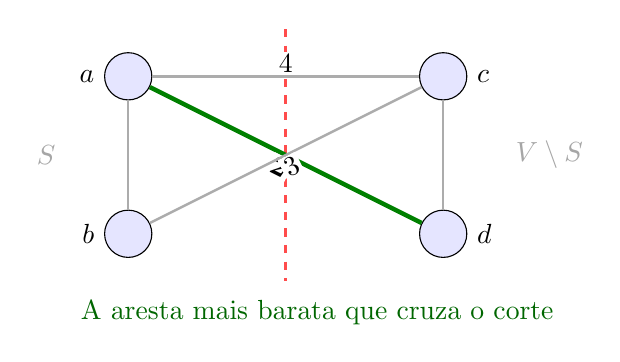
\begin{tikzpicture}[scale=1]
                  % Estilos
                  \tikzset{
                      v/.style={circle, draw, fill=blue!10, minimum size=6mm, inner sep=0pt},
                      edgeG/.style={line width=0.9pt, draw=gray!65},
                      cross/.style={line width=1pt, draw=gray!65},
                      safe/.style={line width=1.6pt, draw=green!50!black},
                      cutline/.style={red!70, dashed, line width=1pt}
                  }
                  % Nós
                  \node[v, label=left:$a$] (A) at (-2, 1) {};
                  \node[v, label=left:$b$] (B) at (-2,-1) {};
                  \node[v, label=right:$c$] (C) at ( 2, 1) {};
                  \node[v, label=right:$d$] (D) at ( 2,-1) {};

                  % Lados do corte (rótulos)
                  \node[anchor=east, gray!70] at (-2.8, 0) {$S$};
                  \node[anchor=west, gray!70] at ( 2.8, 0) {$V\setminus S$};

                  % Linha do corte
                  \draw[cutline] (0, 1.6) -- (0,-1.6);

                  % Arestas internas (apenas contexto)
                  \draw[edgeG] (A) -- (B);
                  \draw[edgeG] (C) -- (D);

                  % Arestas que cruzam o corte (com pesos)
                  \draw[edgeG] (A) -- node[above, sloped, fill=white, inner sep=1pt] {4} (C);
                  \draw[safe]  (A) -- node[below, sloped, fill=white, inner sep=1pt] {\textbf{2}} (D);
                  \draw[edgeG] (B) -- node[below, sloped, fill=white, inner sep=1pt] {3} (C);

                  % Destaque textual
                  \node[green!40!black] at (0.4,-2.0) {A aresta mais barata que cruza o corte};
              \end{tikzpicture}
              \caption{Princípio do corte seguro: entre as arestas que cruzam \((S, V\setminus S)\), a de menor peso (em verde) é \emph{segura} — pode ser incluída em alguma MST sem perder optimalidade.}
              \label{fig:mst-cut-safe}
          \end{figure}
    \item \textbf{Princípio do uso da aresta mais pesada em um ciclo.} Em qualquer \emph{ciclo}, a aresta de maior peso \emph{não} pode pertencer a uma MST, pois existe uma troca que reduz (ou não aumenta) o custo total removendo essa aresta pesada, podemos entender que em um ciclo \(C\), remover a aresta \emph{mais pesada} não desconecta o grafo (há caminho alternativo dentro do próprio ciclo). Como é a mais cara, retirá-la só pode reduzir (ou manter) o custo. Logo, nenhuma MST precisa conter a aresta mais pesada de um ciclo.


          \begin{figure}[H]
              \centering
              \includegraphics[width=0.9\linewidth]{figures/fig_mst_cycle_heavy.pdf}

              \caption{Princípio do ciclo: em qualquer ciclo, a aresta mais pesada (em vermelho) pode ser removida sem desconectar o grafo, reduzindo (ou não aumentando) o custo. Portanto, nenhuma MST contém a aresta mais pesada de um ciclo.}
              \label{fig:mst-cycle-heavy}\end{figure}

\end{itemize}

Assim o problema de encontrar uma árvore geradora mínima (MST) consiste em dado um grafo (não dirigido), conexo e ponderado \(G=(V,E)\) com pesos \(w:E\to\mathbb{R}\), queremos um subconjunto de arestas \(T\subseteq E\) que conecta todos os vértices sem ciclos (forma uma árvore) e minimiza \(\sum_{e\in T} w(e)\).
Com base nos princípios acima, duas soluções gulosas são propostas: \textbf{Kruskal} e \textbf{Prim}.

\begin{itemize}\setlength{\itemsep}{2pt}
    \item \textbf{Kruskal}: ordena as arestas por peso e adiciona enquanto não formar ciclo; usa o princípio do ciclo para evitar carregar a aresta mais pesada de um ciclo.
    \item \textbf{Prim}: começa em um vértice e cresce a árvore; a cada passo escolhe a aresta mais leve que cruza o corte entre “dentro” e “fora” — aplicação direta do princípio do corte.
\end{itemize}


\begin{algobox}{Kruskal (MST, guloso por peso crescente)}{mst-kruskal}
    Entrada: grafo não dirigido \(G=(V,E)\), pesos \(w\).
    \begin{enumerate}\setlength{\itemsep}{2pt}
        \item Ordene as arestas por peso crescente.
        \item Inicialize um \emph{Union-Find}\footnote{Também conhecido como \emph{Disjoint Set Union} (DSU) ou \emph{estrutura de conjuntos disjuntos}. Mantém uma partição dinâmica dos vértices em componentes, oferecendo operações \texttt{find} (descobrir o representante do conjunto) e \texttt{union} (unir dois conjuntos). Com as heurísticas de \emph{união por rank/tamanho} e \emph{compressão de caminhos}, ambas operam em tempo amortizado \(\alpha(n)\) (a função inversa de Ackermann), efetivamente constante na prática. Em Kruskal, essa estrutura detecta ciclos rapidamente ao verificar se as pontas de uma aresta pertencem a componentes distintas.} com cada vértice em seu próprio conjunto; comece com \(T=\emptyset\).
        \item Para cada aresta \(e=\{u,v\}\) na ordem: se \(u\) e \(v\) estão em componentes diferentes, una as componentes e adicione \(e\) a \(T\).
        \item Pare quando \(|T|=|V|-1\). Devolva \(T\).
    \end{enumerate}
\end{algobox}

Kruskal é correto pelos princípios de corte e ciclo; com Union-Find eficiente, roda em \(O(m\log m)\) (ou \(O(m\log n)\)).

\begin{algobox}{Prim (MST, expansão por corte mínimo)}{mst-prim}
    Entrada: grafo não dirigido \(G=(V,E)\), pesos \(w\), vértice inicial \(s\).
    \begin{enumerate}\setlength{\itemsep}{2pt}
        \item Inicialize \(T=\{s\}\) e uma fila de prioridades\footnote{Estrutura que mantém elementos com chaves de prioridade e permite extrair rapidamente o de menor (ou maior) chave. Implementações típicas: \emph{heap} binário (\(\mathrm{push}/\mathrm{decrease\text{-}key}/\mathrm{pop}\) em \(O(\log n)\)), \emph{heap} de Fibonacci (\(\mathrm{decrease\text{-}key}\) amortizado \(O(1)\), \(\mathrm{pop}\) em \(O(\log n)\)), e, em grafos com pesos pequenos, fila bucket (Dial) com tempos quase-lineares. No Prim, a fila é chaveada pelo menor peso de aresta que conecta o vértice fora da árvore ao conjunto \(T\).} com as arestas que saem de \(T\), chaveando pelo menor peso.
        \item Enquanto \(|T|<|V|\): extraia a aresta mais leve \(\{u,v\}\) com \(u\in T\) e \(v\notin T\); adicione \(v\) e \(\{u,v\}\) à árvore; atualize as chaves das arestas que cruzam o novo corte.
        \item Devolva a árvore construída.
    \end{enumerate}
\end{algobox}

Prim também é correto pelo princípio do corte; com fila de prioridades binária, executa em \(O(m\log n)\) (ou em \(O(m+n\log n)\)); em grafos densos com \emph{heaps} de Fibonacci\footnote{\emph{Heaps} (montes) são implementações clássicas de filas de prioridades. O \textbf{heap binário} mantém uma árvore quase completa e executa \texttt{insert}/\texttt{extract-min}/\texttt{decrease-key} em \(O(\log n)\). Já o \textbf{heap de Fibonacci} é uma estrutura amortizada com \texttt{decrease-key} e \texttt{meld} (união) em \(O(1)\) amortizado e \texttt{extract-min} em \(O(\log n)\). Em algoritmos como Prim e Dijkstra, onde \texttt{decrease-key} é frequente, isso leva a \(O(m+n\log n)\). Apesar da melhor garantia assintótica, constantes e implementação mais simples fazem heaps binários (ou \emph{pairing heaps}) serem frequentemente competitivos na prática.}, pode-se obter \(O(m+n\log n)\) \cite{cormen2009,kleinberg2006,west2001introduction,diestel2017graph}.


Os algoritmos gulosos de MST são corretos em grafos não dirigidos, mas a passagem para digrafos \emph{não} é direta. No caso dirigido, buscamos uma \textbf{r-arborescência de custo mínimo}: para cada \(v\neq r\), exatamente um arco entra em \(v\), e o conjunto deve ser acíclico e alcançável a partir de \(r\). Se imitarmos a receita de MST (escolher sempre o arco de entrada mais barato), aparecem \emph{ciclos dirigidos}, e não há um análogo imediato do “corte seguro”.


Duas abordagens clássicas contornam essas dificuldades: (i) \textbf{Chu–Liu/Edmonds}, que mantém \emph{custos reduzidos} (criando arcos de custo reduzido zero) e resolve conflitos por \emph{contração de ciclos}; e (ii) o procedimento em duas fases de \textbf{Frank}, que parte de uma arborescência qualquer e a refina via ajustes de custos e trocas de arcos. Em ambos os casos, escolhas locais são acopladas a um mecanismo global de consistência, garantindo otimalidade no caso dirigido \cite{schrijver2003comb}.

\subsection{A busca em digrafos}


O primeiro avanço significativo na busca por arborescências de custo mínimo em digrafos foi feito por Y. Chu e T. Liu em 1965, que propuseram um algoritmo para encontrar a arborescência de custo mínimo em um digrafo. Esse algoritmo foi posteriormente aprimorado por Jack Edmonds em 1967, que introduziu o conceito de custos reduzidos e a técnica de contração de ciclos, tornando o algoritmo mais eficiente e robusto.


Desde então, a pesquisa nessa área tem se concentrado em melhorar a eficiência dos algoritmos existentes, bem como em explorar novas técnicas e abordagens para lidar com diferentes tipos de digrafos e restrições adicionais. A contribuição de András Frank, que propôs um procedimento em duas fases para encontrar arborescências de custo mínimo, é um exemplo notável dessa evolução contínua.

\section{Os meios para um fim}


Maquiavel é conhecido por uma de suas citações: ``Os fins justificam os meios''. Essa frase ficou famosa porque tem uma interpretação polêmica: em certas circunstâncias, qualquer ação pode ser justificada se o resultado final for considerado positivo ou benéfico. Muitos não concordam com essa visão, argumentando que os meios também importam e que ações imorais não podem ser justificadas por bons resultados.


Por um lado, na matemática essa frase pode ser validada quando falamos em duas formas distintas de construir algoritmos: por \emph{iteratividade} ou \emph{recursividade}.

\subsection{Iteratividade}

Muitos algoritmos — incluindo os gulosos — são construídos por \emph{iteração}: repetimos um bloco de instruções enquanto uma condição não é satisfeita. Para projetar e analisar laços com clareza, três ideias são centrais:

\begin{itemize}\setlength{\itemsep}{2pt}
    \item \textbf{Invariante de laço}: uma propriedade que é verdadeira antes do laço e permanece verdadeira a cada iteração. Ela explica \emph{o que} está sendo mantido correto durante a construção.
    \item \textbf{Variante (medida de progresso)}: uma quantidade que melhora estritamente a cada iteração (ex.: aumenta $|T|$, diminui $|V|$, reduz um potencial). Garante \emph{terminação}.
    \item \textbf{Critério de parada e pós-condição}: quando o laço termina, o invariante implica a especificação desejada.
\end{itemize}


\textit{Na prática.} Em \textbf{Kruskal}, o invariante é “$T$ é uma floresta acíclica e cada componente foi conectado por arestas seguras”; a variante é $|T|$, que cresce até $|V|-1$. Em \textbf{Prim}, “$T$ conecta um conjunto de vértices e as chaves refletem o menor corte atual”; a variante é o tamanho de $T$. Muitas análises usam \emph{custo por iteração} ou \emph{análise amortizada}\footnote{A análise amortizada distribui o custo de operações caras sobre uma sequência, garantindo um custo médio por operação (ex.: \texttt{decrease-key} em heaps de Fibonacci).} para capturar o desempenho agregado.

\subsubsection{Recursividade}

Recursão resolve instâncias grandes chamando o próprio algoritmo em subinstâncias menores. Um projeto claro inclui:

\begin{itemize}\setlength{\itemsep}{2pt}
    \item \textbf{Casos base}: instâncias mínimas resolvidas diretamente.
    \item \textbf{Passo recursivo}: como decompor e combinar soluções dos subproblemas.
    \item \textbf{Medida decrescente}: uma grandeza que estritamente diminui a cada chamada (ex.: número de vértices após contração), assegurando terminção.
    \item \textbf{Corretude por indução}: assumimos corretas as chamadas recursivas (hipótese indutiva) e provamos que a combinação produz uma solução correta.
    \item \textbf{Custo por recorrência}: tempo expresso por $T(n)$ e resolvido por \emph{árvore de recursão} ou Teorema Mestre\footnote{Esboço: quando $T(n)=a\,T(n/b)+f(n)$, com $a\ge 1$, $b>1$, comparamos $f(n)$ a $n^{\log_b a}$. Não é necessário aqui, mas a técnica guia estimativas assintóticas.}.
\end{itemize}


\textit{Na prática.} Em \textbf{Chu–Liu/Edmonds}, o passo recursivo contrai um ciclo dirigido e ajusta custos; a medida decrescente é $|V|$ (a cada contração reduzimos o número de vértices do problema), e a expansão final preserva otimalidade. No procedimento em duas fases de \textbf{Frank}, a primeira fase produz uma arborescência inicial; a segunda aplica \emph{refinamentos iterativos} guiados por custos reduzidos — um exemplo de mistura entre recursão estrutural e iteração local.


Para ilustrar, resolvemos o mesmo problema — calcular o fatorial \(n!\) — de forma \emph{iterativa} e \emph{recursiva}.

\begin{algobox}{Fatorial (iterativo)}{fatorial-iterativo}
    Entrada: inteiro \(n\ge 0\)
    \begin{enumerate}\setlength{\itemsep}{2pt}
        \item Se \(n=0\), devolva \(1\).
        \item Defina \(r\leftarrow 1\).
        \item Para \(i\) de \(1\) até \(n\): \(r\leftarrow r\cdot i\).
        \item Devolva \(r\).
    \end{enumerate}
\end{algobox}

\begin{algobox}{Fatorial (recursivo)}{fatorial-recursivo}
    Entrada: inteiro \(n\ge 0\)
    \begin{enumerate}\setlength{\itemsep}{2pt}
        \item Se \(n\le 1\), devolva \(1\). \hfill (caso base)
        \item Caso contrário, devolva \(n\cdot \textsc{Fatorial}(n-1)\). \hfill (passo recursivo)
    \end{enumerate}
\end{algobox}


Ambas as versões computam a mesma função. A iterativa evidencia a \emph{variante} (o contador \(i\)) e um \emph{invariante} simples (\(r= i!\) ao fim da iteração \(i\)); a recursiva explicita o \emph{caso base} e o \emph{passo indutivo}, e corresponde, operacionalmente, a empilhar chamadas com parâmetros decrescentes até \(n=1\).


Existe inclusive uma prova matemática\footnote{Em modelos padrão de computação (máquinas de Turing, RAM), \emph{iteração} e \emph{recursão} têm o mesmo poder expressivo: laços podem ser reescritos como recursão (sobre um contador/estado) e chamadas recursivas podem ser eliminadas por uma simulação explícita da pilha (iteração com uma estrutura \textit{stack}). Demonstrações e variantes aparecem em textos clássicos de teoria da computação e projeto de algoritmos; ver, por exemplo, \cite{cormen2009} (eliminação de recursão via pilha explícita). Aqui registramos apenas a equivalência conceitual, sem apresentá-la.} que diz que qualquer algoritmo iterativo pode ser reescrito de forma recursiva, e vice-versa. Ou seja, \emph{os fins justificam os meios}: a escolha entre iteração e recursão é muitas vezes uma questão de preferência ou conveniência, já que ambos podem alcançar o mesmo objetivo. Porém, algoritmos recursivos podem ser mais elegantes e fáceis de entender, enquanto algoritmos iterativos podem ser mais eficientes em termos de uso de memória (evitando a sobrecarga da pilha de chamadas). Ou seja, os meios também importam. E os trabalhos de Chu–Liu/Edmonds e Frank ilustram bem essa tensão:
\begin{itemize}\setlength{\itemsep}{2pt}
    \item \textbf{Chu–Liu/Edmonds} é um algoritmo recursivo que contrai ciclos e resolve o problema em subinstâncias menores, usando custos reduzidos para manter a otimalidade.
    \item O procedimento em \textbf{Frank} é iterativo, começando com uma arborescência qualquer e refinando-a por trocas locais guiadas por custos reduzidos, até alcançar a otimalidade.
\end{itemize}
Ambos os algoritmos são corretos e eficientes, mas adotam meios diferentes para alcançar o mesmo fim: encontrar uma r-arborescência de custo mínimo em um digrafo ponderado.


Antes de entrar nos detalhes, faremos uma breve revisão dos conceitos e técnicas que utilizaremos adiante, para uniformizar a notação e tornar a leitura mais fluida.

\subsubsection{Revisão: conceitos fundamentais e técnicas}


Antes de mergulharmos nos algoritmos específicos, é importante revisitar alguns conceitos fundamentais que serão cruciais para nossa compreensão:

\subsubsection{Conceitos Fundamentais:}
\begin{itemize}\setlength{\itemsep}{2pt}
    \item \textbf{digrafo}: um grafo direcionado onde os arcos têm uma direção específica, indo de um vértice a outro.
    \item \textbf{Arborescência}: uma árvore direcionada onde todos os caminhos partem de um vértice raiz e alcançam todos os outros vértices.
    \item \textbf{Custo dos Arcos}: cada arco em um digrafo pode ter um custo associado, representando, por exemplo, o custo de transporte ou a distância.
    \item \textbf{r-Arborescência de Custo Mínimo}: uma arborescência enraizada em um vértice \(r\) que minimiza a soma dos custos dos arcos que a compõem.
    \item \textbf{Cortes e Conectividade}: a importância dos cortes em digrafos para garantir a conectividade e a existência de arborescências.
    \item \textbf{Condicionalidade de Fulkerson}: as condições necessárias e suficientes para a existência de uma r-arborescência de custo mínimo.
\end{itemize}

\subsubsection{Técnicas e Abordagens:}

Para encontrar r-arborescências de custo mínimo, utilizaremos algumas técnicas e abordagens específicas:
\begin{itemize}\setlength{\itemsep}{2pt}
    \item \textbf{Normalização de Custos}: ajustaremos os custos dos arcos para facilitar a identificação de arcos de custo reduzido zero.
    \item \textbf{Contração de Ciclos}: quando formos encontrar ciclos de arcos de custo reduzido zero, os contrairemos para simplificar o digrafo.
    \item \textbf{Custos Reduzidos}: utilizaremos custos reduzidos para identificar arcos que podem ser incluídos na arborescência sem aumentar o custo total.
    \item \textbf{Estratégias Gulosas}: aplicaremos estratégias gulosas para selecionar arcos de forma eficiente, garantindo que cada escolha local contribua para a solução global ótima.
    \item \textbf{Recursão e Expansão}: usaremos recursão para resolver subproblemas em digrafos contraídos e expandiremos as soluções para o digrafo original.
    \item \textbf{Análise de Complexidade}: avaliaremos a eficiência dos algoritmos em termos de tempo e espaço, garantindo que sejam viáveis para grandes digrafos.
    \item \textbf{Provas de Corretude}: forneceremos argumentos formais para garantir que os algoritmos realmente produzem a r-arborescência de custo mínimo.
\end{itemize}


No capítulo seguinte, detalharemos o algoritmo de Chu–Liu/Edmonds, bem como os detalhes da implementação em Python; o subsequente será dedicado ao procedimento em duas fases de Frank e à respectiva implementação.
